\section{退化的处理}
\label{sec:simplex-degeneracy}

定理~\ref{thm:simplex-finite-nondegenerate}的有限终止依赖一个假设：每次换基都能真正走出去。本节研究这个假设不成立时算法会发生什么，以及怎样修补。

\paragraph{同一个顶点，不同的基}
把工厂的工时从$10$改成$7$，三条约束边界就同时经过点$(2,3)$，如图~\ref{fig:simplex-degenerate-vertex}(a)所示。二维平面上确定一个点只需要两条线，这里却有三条，选哪两条都行。对应到代数上，这个点的$x_3=x_4=x_5=0$，三个变量中必须有一个留在基中，取值为零。这就是退化：一个基本可行解有基变量取零，同一个点可以对应多个基。

\begin{BookInlineFigure}
 \centering
 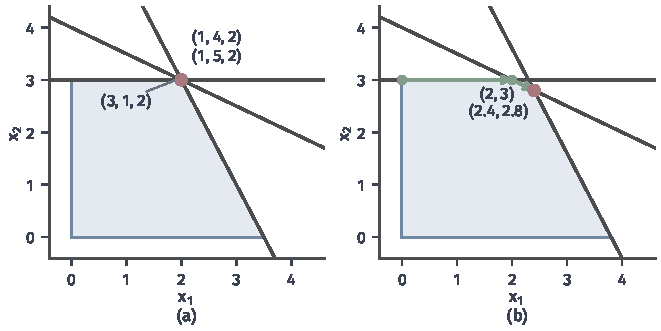
\includegraphics[width=112mm]{figures/05-optimization/01-linear-programming/matplotlib/simplex-degenerate-vertex/figure.pdf}
 \caption{退化顶点及其扰动。(a)~工时取$7$时三条约束边界（深灰）交于红点$(2,3)$，旁边的三元组是对应这同一个点的三个基。(b)~把工时夸张地增大到$7.6$后，这个顶点分裂成$(2,3)$和$(2.4,2.8)$两个相邻顶点，绿色路径多走一条真实的短边，每步都有实际移动。}
 \label{fig:simplex-degenerate-vertex}
\end{BookInlineFigure}

\paragraph{不移动的换基}
从基$(3,4,5)$开始运行Dantzig规则，前一轮与之前相同，$x_2$入基，点到$(0,3)$，基是$(3,4,2)$，$\bm{x}_B=(2,4,3)^\top$。下一轮$x_1$入基，$\bm{u}=(1,2,0)^\top$，两个比值并列：
\[
 \frac{2}{1}=2,\qquad \frac{4}{2}=2.
\]
这里的并列正是退化的来源：两个基变量同时降到零，只有一个能出基，另一个留下来取零。按下标小的规则，$x_3$出基，得到
\[
 B=(1,4,2),\qquad \bm{x}_B=(2,0,3)^\top,\qquad f=-23,
\]
点到达$(2,3)$。

此时的对偶候选和约化成本是
\[
 \bm{y}=(-4,0,3)^\top,\qquad s_3=4,\qquad s_5=-3.
\]
$s_5<0$，判别说还不能停。$x_5$入基，$\bm{u}=(-2,3,1)^\top$，比值是
\[
 \frac{x_4}{u_2}=\frac{0}{3}=0,\qquad \frac{x_2}{u_3}=\frac{3}{1}=3.
\]
步长$\alpha=0$，基变成$(1,5,2)$，点和目标都没变。新基的对偶候选和约化成本是
\[
 \bm{y}=(-2,-1,0)^\top,\qquad s_3=2,\qquad s_4=1,
\]
全部非负，算法才停下。

其实$(2,3)$早已是最优点，这一轮换基只是把基换成能出示证书的那一个。如果上一轮并列时让$x_4$出基，就直接得到基$(3,1,2)$，此时$\bm{y}=(0,-2,-3)^\top$，$s_4=2$，$s_5=3$，立即停止。这说明两点：退化基上$s_j<0$并不表示当前点不是最优；证书依赖基，同一个最优点上有的基能给出证书，有的基不能。

\paragraph{循环}
既然目标可以不下降，“每步都变好”的论证就失效了，算法可能在一组基之间兜圈子，这称为\term{循环}（cycling）。下面是一个有三行四个决策变量的例子，$x_5,x_6,x_7$是松弛变量：
\begin{equation}
 \begin{aligned}
 \min\quad & -10x_1+57x_2+9x_3+24x_4\\
 \text{s.t.}\quad & \tfrac12x_1-\tfrac{11}{2}x_2-\tfrac52x_3+9x_4+x_5=0,\\
 & \tfrac12x_1-\tfrac32x_2-\tfrac12x_3+x_4+x_6=0,\\
 & x_1+x_7=1,\qquad \bm{x}\geq\bm{0}.
 \end{aligned}
 \label{eq:simplex-cycling-example}
\end{equation}
用Dantzig规则，比值并列时取下标最小者，从基$(5,6,7)$出发，得到表~\ref{tab:simplex-cycling-rounds}的序列。每一步都有负的约化成本，每一步的步长都是零，第$6$步回到起点。

\begin{BookInlineTable}
 \centering
 \begin{tabular}{ccccc}
  \toprule
  $t$ & $B^{(t)}$ & 入基 & 约化成本 & 出基\\
  \midrule
  $0$ & $(5,6,7)$ & $x_1$ & $-10$ & $x_5$\\
  $1$ & $(1,6,7)$ & $x_2$ & $-53$ & $x_6$\\
  $2$ & $(1,2,7)$ & $x_3$ & $-29/2$ & $x_1$\\
  $3$ & $(3,2,7)$ & $x_4$ & $-18$ & $x_2$\\
  $4$ & $(3,4,7)$ & $x_5$ & $-21/2$ & $x_3$\\
  $5$ & $(5,4,7)$ & $x_6$ & $-24$ & $x_4$\\
  $6$ & $(5,6,7)$ & 回到第$0$轮 & & \\
  \bottomrule
 \end{tabular}
 \caption{问题~\eqref{eq:simplex-cycling-example}在Dantzig规则下的循环。}
 \label{tab:simplex-cycling-rounds}
\end{BookInlineTable}

图~\ref{fig:simplex-cycle-bases}把这六个基画成一个环。这个环上$\bm{x}$从未变化，所以只看目标值的话，看不出算法在做什么。

\begin{BookInlineFigure}
 \centering
 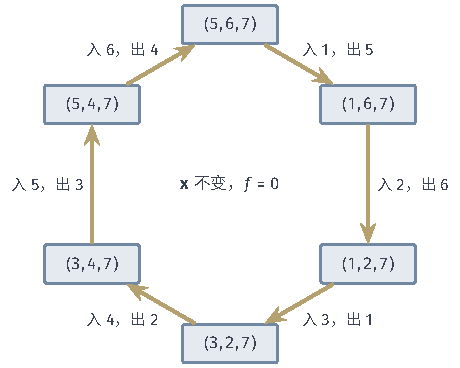
\includegraphics[width=78mm]{figures/05-optimization/01-linear-programming/tikz/simplex-cycle-bases/figure.pdf}
 \caption{问题~\eqref{eq:simplex-cycling-example}的六个基组成的循环。方框是基，黄色箭头是Dantzig规则下的一次换基，箭头旁写明入基和出基下标。整个环上$\bm{x}$和目标值都不变。}
 \label{fig:simplex-cycle-bases}
\end{BookInlineFigure}

\paragraph{Bland规则}
要打破循环，只需把“选哪一个”的自由度用一条固定的规则收走。\term{Bland规则}（Bland's rule）规定：入基变量取所有$s_j<0$中下标最小的；比值检验并列时，出基变量取下标最小的\scite{math-bland1977finite}。

\begin{theorem}[Bland规则的有限终止]
 \label{thm:simplex-bland}
 在精确算术下，使用Bland规则的单纯形法不会循环，因而经过有限次换基后停止。
\end{theorem}

\begin{proof}
 假设出现循环。目标值不增，循环中目标必须保持不变，所以每一步的步长都是零，$\bm{x}$在整个循环中不变，记为$\bar{\bm{x}}$。

 称循环中曾经入基的下标为活跃下标，活跃下标也必定曾经出基。活跃下标在某个基中非基，所以对应的$\bar{x}_j=0$。设$k$是最大的活跃下标。取循环中$k$将要出基的一个基$B$，此时入基的是活跃下标$q<k$。再取循环中$k$将要入基的一个基$B'$，其约化成本记为$\bm{s}'$，对偶候选记为$\bm{y}'$。

 由基$B$和入基$q$按式~\eqref{eq:simplex-direction}构造方向$\bm{d}$，它满足
 \[
  \bm{A}\bm{d}=\bm{0},\qquad \bm{c}^\top\bm{d}=s_q<0.
 \]
 用$\bm{s}'=\bm{c}-\bm{A}^\top\bm{y}'$，得到
 \[
  (\bm{s}')^\top\bm{d}=\bm{c}^\top\bm{d}-(\bm{y}')^\top\bm{A}\bm{d}=s_q<0.
 \]
 因此存在下标$j$使$s'_jd_j<0$。

 这个$j$满足$j\notin B'$，因为$B'$的基变量$s'_j=0$；同时$d_j\neq0$，故$j\in B$或$j=q$。两种情况下$j$都在循环中某一时刻属于基或正要入基，而在$B'$非基，所以$j$是活跃下标，$j\leq k$。

 下面排除$j=k$。$k$在$B$中将要出基，说明$u_k>0$，$d_k<0$；而$k$在$B'$中将要入基，说明$s'_k<0$。于是$s'_kd_k>0$，所以$j\neq k$，只能$j<k$。

 Bland规则在$B'$选了$k$入基，这说明比$k$小的下标都没有负的约化成本，所以$s'_j\geq0$，结合$s'_jd_j<0$得到$s'_j>0$，$d_j<0$。特别地$j\neq q$，所以$j\in B$，且$u_j=-d_j>0$。又$j$活跃，$\bar{x}_j=0$，于是$j$的比值是$0$，与$k$的比值并列。$j<k$却没有被选中出基，这与Bland规则矛盾。

 不循环意味着基不重复，基的个数有限，所以换基只能进行有限次。
\end{proof}

证明的结构值得留意：用最大的活跃下标构造一个对偶上的矛盾，正是“取下标最小”这个规则使矛盾成立。这个规则的作用是保证有限，不是追求速度，它常常比Dantzig规则走更多步。

回到问题~\eqref{eq:simplex-cycling-example}，Bland规则的前$5$步与表~\ref{tab:simplex-cycling-rounds}相同。第$5$轮基是$(5,4,7)$，约化成本$s_1=-22$，$s_6=-24$。Dantzig规则选$s_6$回到起点，Bland规则选下标小的$x_1$，走出了循环。再换一次基后，$x_3$入基时唯一的比值来自$x_7$，$\alpha=1$，得到
\[
 \bm{x}=(1,0,1,0,2,0,0)^\top,\qquad f=-1,
\]
约化成本全部非负。图~\ref{fig:simplex-cycling-objective}对比了两种规则的目标值。

\begin{BookInlineFigure}
 \centering
 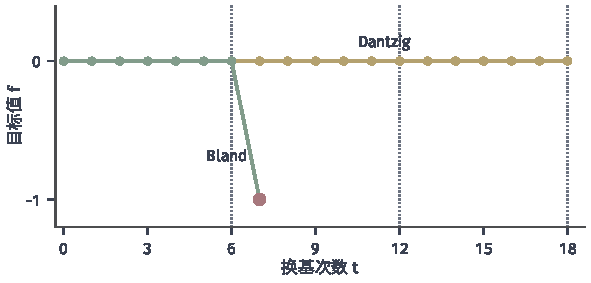
\includegraphics[width=100mm]{figures/05-optimization/01-linear-programming/matplotlib/simplex-cycling-objective/figure.pdf}
 \caption{问题~\eqref{eq:simplex-cycling-example}上两种规则的目标值。黄线是Dantzig规则，目标值恒为$0$，竖直点线标出每$6$步回到起始基；绿线是Bland规则，$6$次零步之后第$7$次换基走到红色的最优点，$f=-1$。}
 \label{fig:simplex-cycling-objective}
\end{BookInlineFigure}

\paragraph{字典序规则}
图~\ref{fig:simplex-degenerate-vertex}(b)提示了另一条路：既然麻烦来自几条约束恰好相交于一点，就把右端轻轻推开，让退化顶点裂成几个相距很近的普通顶点。把右端换成
\[
 \bm{b}+(\epsilon,\epsilon^2,\ldots,\epsilon^m)^\top,
\]
其中$\epsilon>0$充分小，比值并列就不会发生，每步都有严格的下降。

\term{字典序规则}（lexicographic rule）把这个想法做成不需要真的取$\epsilon$的规则：比值并列时，比较各并列行的向量$[\bar{x}_{B(i)},(\bm{A}_B^{-1})_{i,:}]/u_i$，取字典序最小者出基。它的作用等同于对无穷小的扰动做比值检验。证明需要跟踪各行字典序为正这一性质，并说明每次换基使目标行严格字典序下降，读者可查阅线性规划专著\scite{math-bertsimas1997linear}。结论同样是：在精确算术下不循环，有限终止。

两种规则的保证都建立在精确算术之上。浮点计算里，“恰好是零”没有意义，比值并列要用容差判断，舍入误差也会把退化基上的零扰动成微小的正负数。所以实现时除了防循环的规则，还要在最后重新核查可行性和约化成本，第~\ref{sec:simplex-revised}节将说明怎样做。
